\documentclass[11pt]{beamer}
\usepackage{listings} % Include the listings-package
\usepackage[T1]{fontenc}
\usepackage[utf8]{inputenc}
\usepackage[english]{babel}
\usepackage{amsmath}
\usepackage{amssymb, amsfonts, latexsym, cancel}
\usepackage{float}
\usepackage{graphicx}
\usepackage{epstopdf}
\usepackage{subfigure}
\usepackage{hyperref}
%\usepackage{authblk}
\usepackage{blindtext}
\usepackage{booktabs} % Allows the use of \toprule, 
\usepackage{filecontents}
\usepackage{ragged2e}
\usepackage{courier} %% Sets font for listing as Courier.
\usepackage{listings}
%\usepackage{listings, xcolor}
\lstset{
tabsize = 2, %% set tab space width
showstringspaces = false, %% prevent space marking in strings, string is defined as the text that is generally printed directly to the console
numbers = left, %% display line numbers on the left
commentstyle = \color{green}, %% set comment color
keywordstyle = \color{blue}, %% set keyword color
stringstyle = \color{red}, %% set string color
rulecolor = \color{black}, %% set frame color to avoid being affected by text color
basicstyle = \small \ttfamily , %% set listing font and size
breaklines = true, %% enable line breaking
numberstyle = \tiny,
}
\usepackage{caption}
\DeclareCaptionFont{white}{\color{white}}
\DeclareCaptionFormat{listing}{\colorbox{gray}{\parbox{\textwidth}{#1#2#3}}}
\captionsetup[lstlisting]{format=listing,labelfont=white,textfont=white}
\definecolor{urlColor}{rgb}{0.06, 0.3, 0.57}
\definecolor{linkColor}{rgb}{0.57, 0.0, 0.04}
\definecolor{fileColor}{rgb}{0.0, 0.26, 0.26}
\hypersetup{
    colorlinks=true,
    linkcolor=linkColor,
    filecolor=fileColor,      
    urlcolor=urlColor,
}
\urlstyle{same}
\setbeamercovered{transparent}
%\usetheme{Boadilla}
\usetheme{CambridgeUS}
%\usetheme{Berkeley}
%\usetheme{Warsaw}
%\usetheme{Madrid}

\title[Presentación]{\bf\Huge Diseño de software interactivo educativo inclusivo }
\subtitle{HCI-2020}

\author[Grupo 10]
{
    Deyson Victor Diaz Ticona, 
    Kevin Yunior Ccorimanya Paucar, 
    Denilson Flores Valdivia,
    Marco Antonio Ponce de Leon 
}
\institute[UNSA]
{
\inst{1}% 
System Engineering School\\
System Engineering and Informatic Department\\
Production and Services Faculty\\
San Agustin National University of Arequipa
}

\date[2020-10-06]{\scriptsize{2020-10-06}}
\logo{
\includegraphics[width=3.0cm]{logo_unsa.jpg}}
%\titlegraphic{
\includegraphics[width=1.0cm]{logo_unsa.jpg}}

\begin{document}

\begin{frame}
\titlepage
\end{frame}

\begin{frame}
\frametitle{Contenido}
\tableofcontents
\end{frame}

%-------------------------------------------------------------------------------

\section{Introduccion y Problematica}
\begin{frame}
\frametitle{Introduccion y Problematica}
\begin{itemize}
\item Analizar cómo el {\bf usuario} utiliza la {\bf tecnología}, y cómo esta tecnología se adapta a las {\bf necesidades del usuario}.
\end{itemize}
\end{frame}

\section{Enfoque metodologico del diseño}
\begin{frame}
\frametitle{Adecuación en los Recursos Educativos}
    \justify
    \begin{minipage}[c]{0.4\textwidth} 
    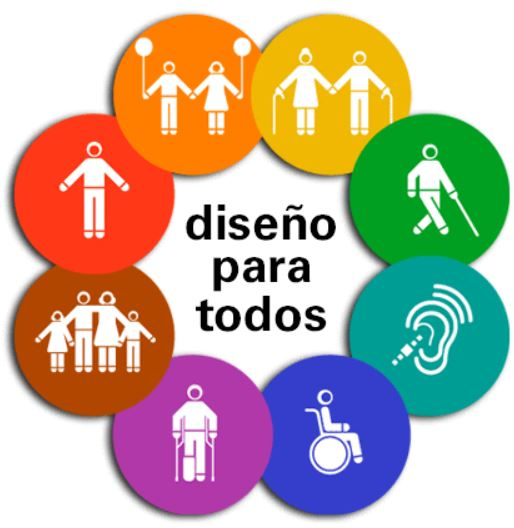
\includegraphics[width=4.5cm, height=6cm]{imagen1.jpg} 
    \end{minipage}
    \begin{minipage}[c]{0.55\textwidth}
        \begin{itemize}
        \item En una escuela inclusiva, deben diseñarse recursos que estén adaptados de manera que puedan ser utilizados y captados por todo el alumnado.
        \item Deben contener estímulos multisensoriales y permitir la accesibilidad a todo el alumnado.
        \end{itemize}
        Las aplicaciones interactivas pueden mejorar la competencia básicas en los niños con dificultad de aprendizaje.
    \end{minipage}
\end{frame}

\begin{frame}
\frametitle{Deficit de aprendizaje versus función cognitiva}
    \begin{figure}
    \centering
     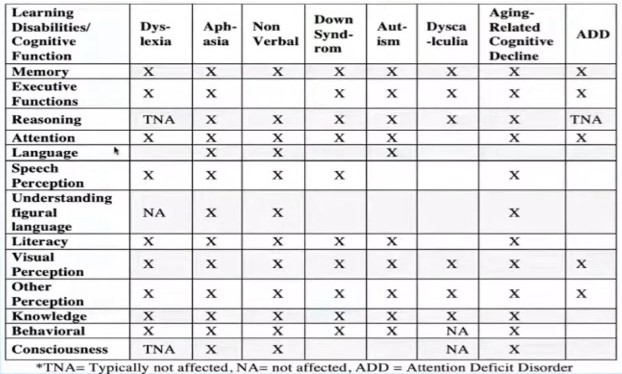
\includegraphics[width=0.8\textwidth]{imagen2.jpg} 
    \end{figure}
\end{frame}

\begin{frame}
\frametitle{Estudiantes de USAER Aguascalientes}
    \begin{figure}
    \centering
     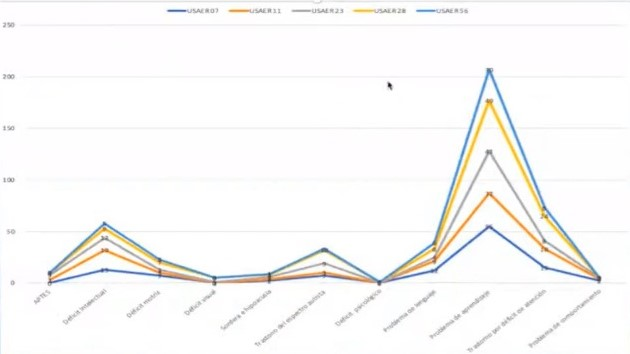
\includegraphics[width=0.8\textwidth]{imagen3.jpg} 
    \end{figure}
\end{frame}

\begin{frame}
\frametitle{Libros del Ministerio de Mexico}
    \begin{figure}
    \centering
     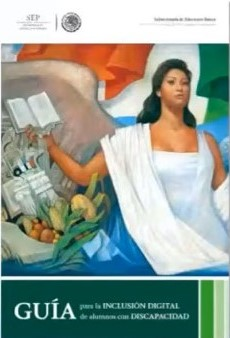
\includegraphics[width=4.0cm]{imagen4-1.jpg}
     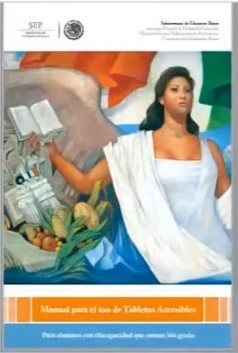
\includegraphics[width=4.0cm]{imagen4-2.jpg}
    \end{figure}
\end{frame}

\begin{frame}
\frametitle{¡¡ Existe una gran cantidad de aplicaciones educativas en linea !!}
    \begin{figure}
    \centering
     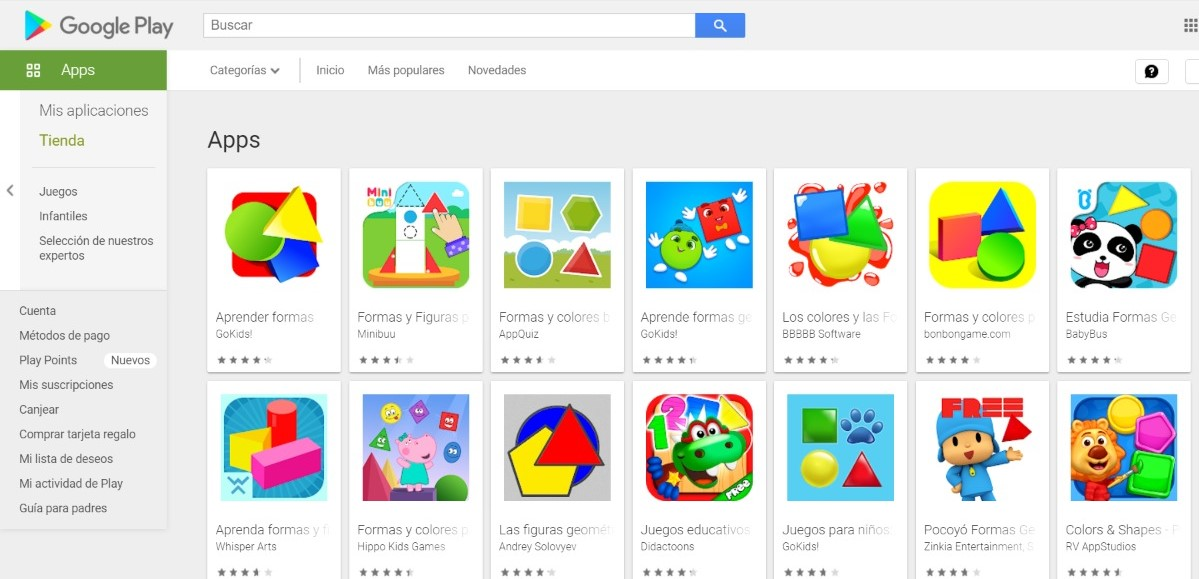
\includegraphics[width=6.0cm]{imagen5-1.jpg}
     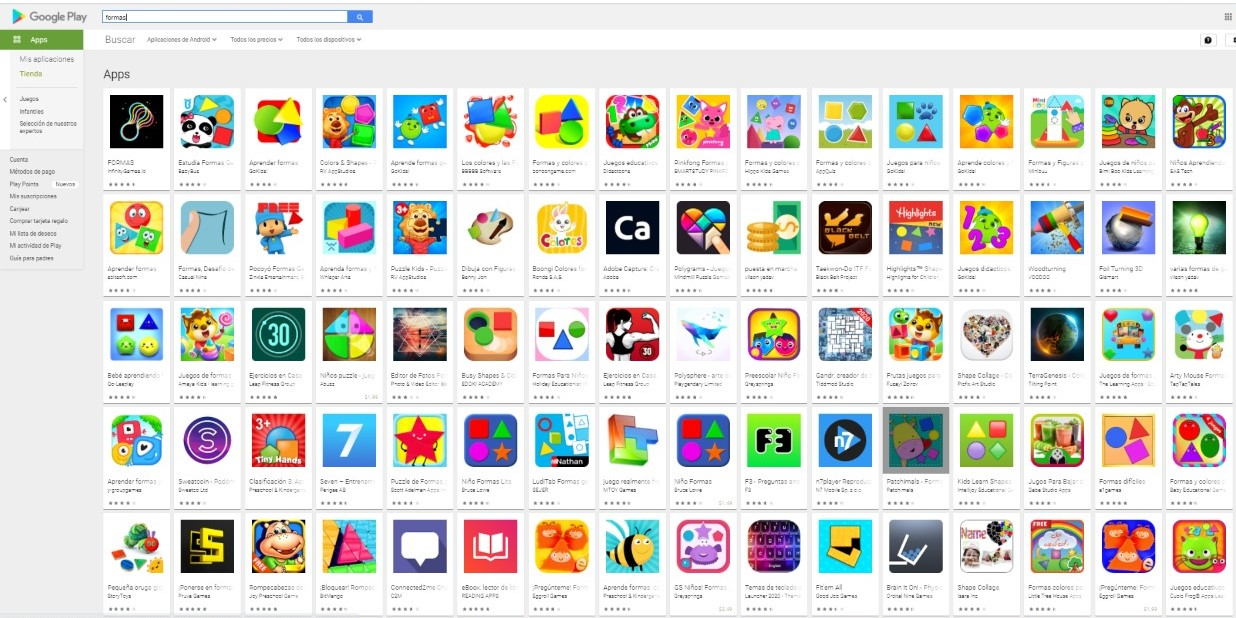
\includegraphics[width=6.0cm]{imagen5-2.jpg}
    \end{figure}
\end{frame}

\begin{frame}
\frametitle{Repositorio de aplicaciones educativas}
    \begin{figure}
    \centering
     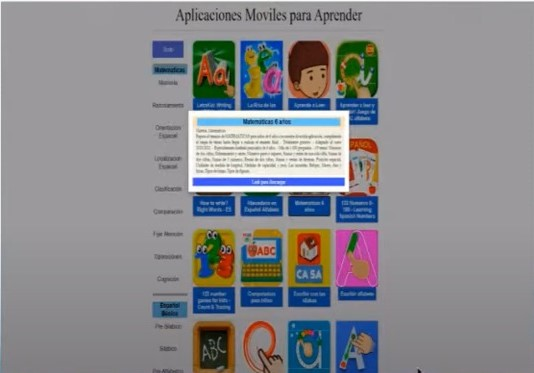
\includegraphics[width=0.8\textwidth]{imagen6.jpg}
    \end{figure}
\end{frame}

\begin{frame}
\frametitle{Ecosistema de apoyo a usuarios con déficit de aprendizaje}
    \begin{figure}
    \centering
     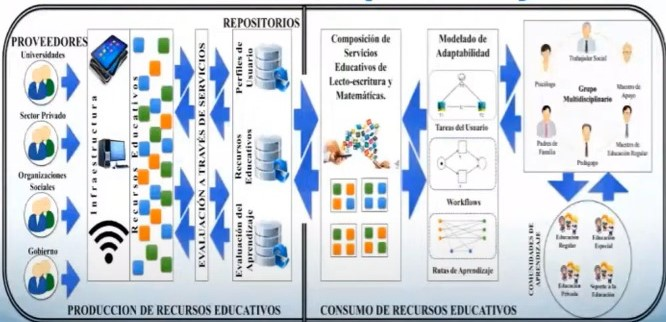
\includegraphics[width=0.8\textwidth]{imagen7.jpg}
    \end{figure}
\end{frame}

\begin{frame}
\frametitle{Compocision de servicios educativos}
    \justify
    Una vez que clasificados, filtrados y almacenados los recursos educativos, algunas veces es necesario agrupar aquellos recursos que a consideración del grupo multidisciplinario pueden ayudar a mitigar las problemáticas de los individuos de las comunidades y esos mismos recursos educativos pueden conformar otra agrupación para mitigar otras necesidades, es decir son altamente reutilizables para problemáticas detectadas.
    \par
    \begin{figure}
    \centering
     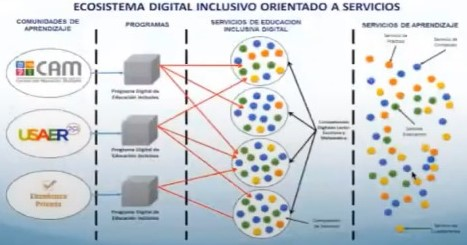
\includegraphics[width=0.7\textwidth]{imagen8.jpg}
    \end{figure}
\end{frame}

\begin{frame}
\frametitle{Modelo de contenido para aplicaciones educativas}
    \begin{figure}
    \centering
     
\includegraphics[width=0.9\textwidth]{imagen9.jpg}
    \end{figure}
\end{frame}

\begin{frame}
\frametitle{Producción colaborativa de recursos educativos}
    \begin{figure}
    \centering
     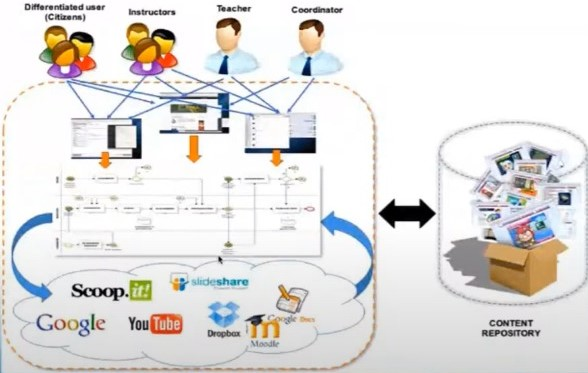
\includegraphics[width=0.7\textwidth]{imagen10.jpg}
    \end{figure}
\end{frame}

\begin{frame}
\frametitle{Catalogo de patrones sobre las aplicaciones educativas}
    \begin{figure}
    \centering
     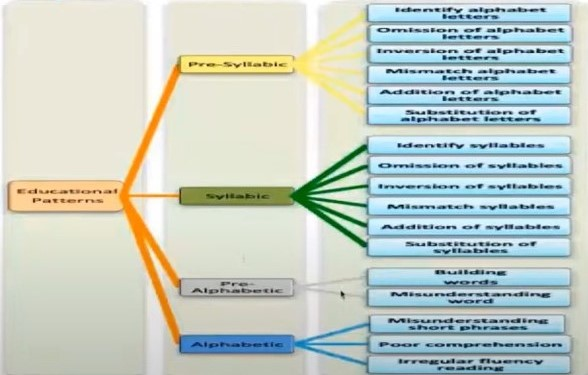
\includegraphics[width=0.7\textwidth]{imagen11.jpg}
    \end{figure}
\end{frame}

\begin{frame}
\frametitle{Identify syllables}
    \begin{figure}
    \centering
     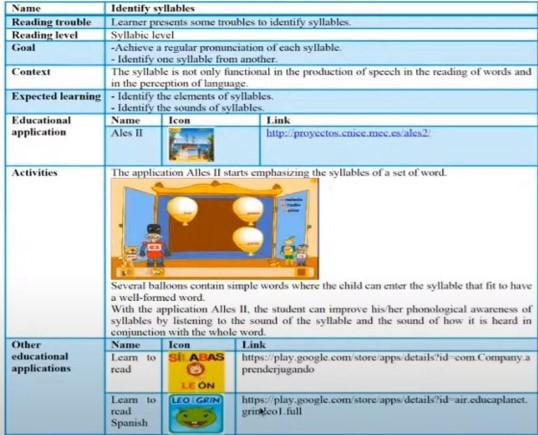
\includegraphics[width=0.7\textwidth]{imagen12.jpg}
    \end{figure}
\end{frame}

\begin{frame}
\frametitle{Misundertanding Simple Phraces}
    \begin{figure}
    \centering
     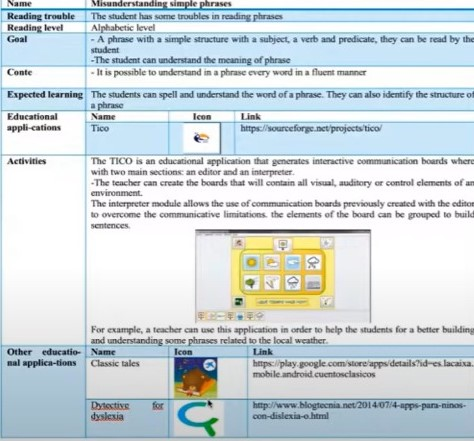
\includegraphics[width=0.6\textwidth]{imagen13.jpg}
    \end{figure}
\end{frame}

\begin{frame}
\frametitle{Modelo de procesos para desarrollar aplicaciones educativas}
    \begin{figure}
    \centering
     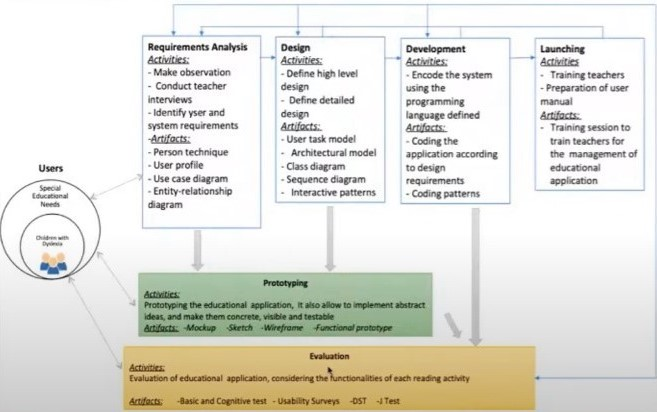
\includegraphics[width=0.8\textwidth]{imagen14.jpg}
    \end{figure}
\end{frame}

%-------------------------------------------------------------------------------

\section{Experiencia en apoyo a aprendizaje inclusivo de la lectura}
\title{Experiencia en lectura}
\begin{frame}
\frametitle{Experiencia en apoyo a aprendizaje inclusivo de la lectura}
    \justify
    Para el aprendizaje inclusivo en la lectura de los niños con problemas de aprendizaje, se dan algunas experiencias impuestas en la Conferencia de IHC, el cual lo explica detalladamente el Dr. Jaime Muñoz Arteaga.
\end{frame}

\begin{frame}
\frametitle{Participantes en el aprendizaje inclusivo de los niños}
    \justify
    \begin{minipage}[c]{0.4\textwidth} 
    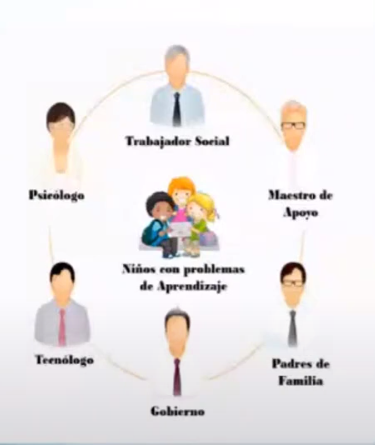
\includegraphics[width=4.8cm, height=6.5cm]{ImagenLectura1.2.png} 
    \end{minipage}
    \begin{minipage}[c]{0.55\textwidth}
        El grupo multidisciplinario de USAER conformado para este caso de estudio estuvo conformado por la maestra de educación regular, la maestra de apoyo, un psicólogo, un trabajador social y un pedagogo, dicha participación de estos actores contribuyó a la generación de un perfil pedagógico, generación de rutas de aprendizaje específicas para los niños, evaluaciones acorde a su  perfil y la interpretación de la retroalimentación para 2 niños daban a través del uso de los recursos educativos.
    \end{minipage}
\end{frame}

\begin{frame}
\frametitle{Perfil de usuario}
    \begin{figure}
    \centering
     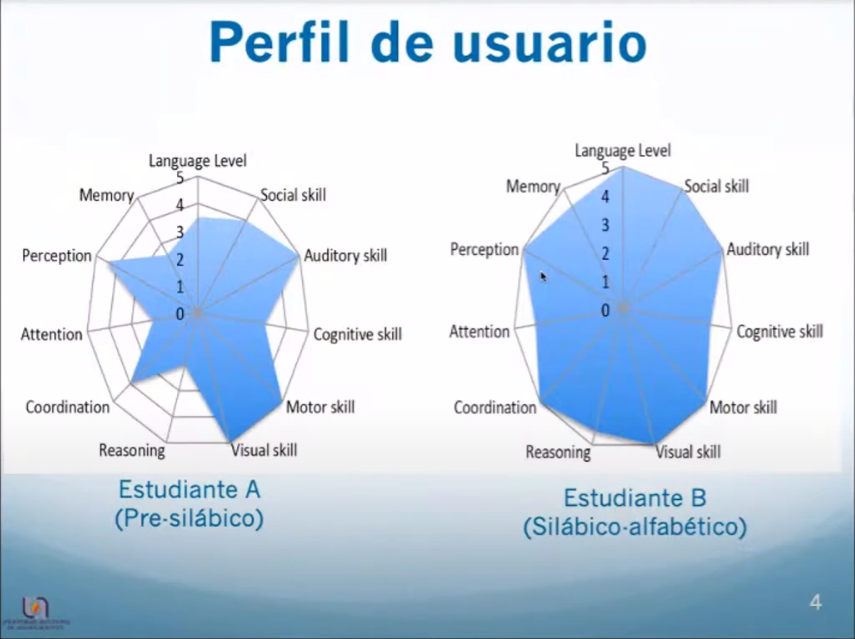
\includegraphics[width=0.8\textwidth]{ImagenLectura2.png}
    \end{figure}
\end{frame}

\begin{frame}
\frametitle{Diagnóstico}
    \begin{figure}
    \centering
     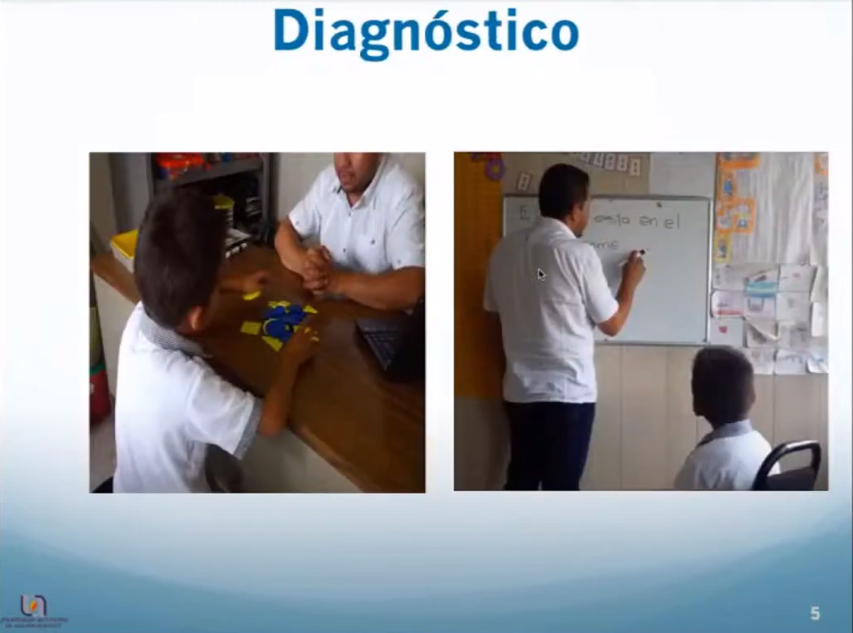
\includegraphics[width=0.8\textwidth]{ImagenLectura3.png}
    \end{figure}
\end{frame}

\begin{frame}
\frametitle{Niveles de Habilidad en la LectoEscritura}
    \begin{figure}
    \centering
     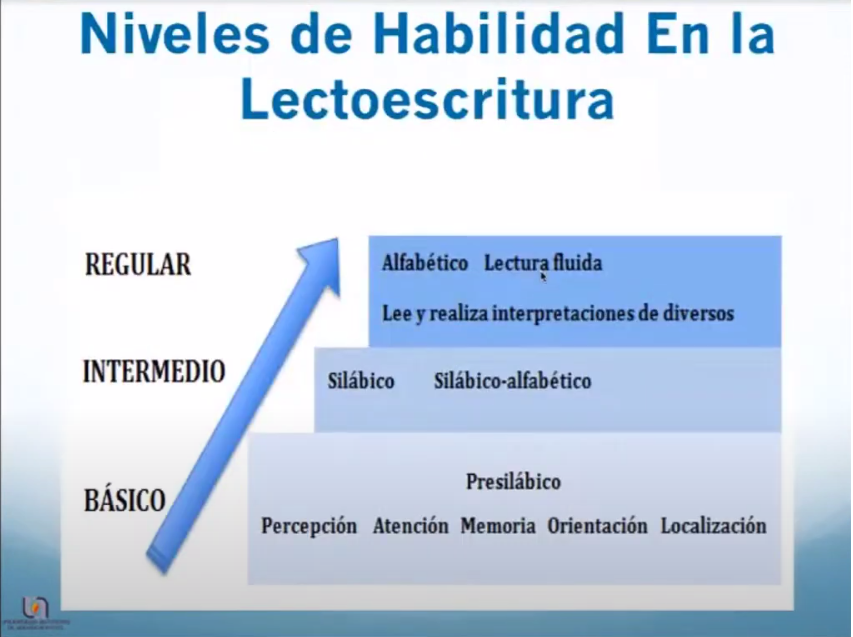
\includegraphics[width=0.8\textwidth]{ImagenLectura4.png}
    \end{figure}
\end{frame}

\begin{frame}
\frametitle{Prototipo de aplicaciones educativas para lectura}
    \begin{figure}
    \centering
     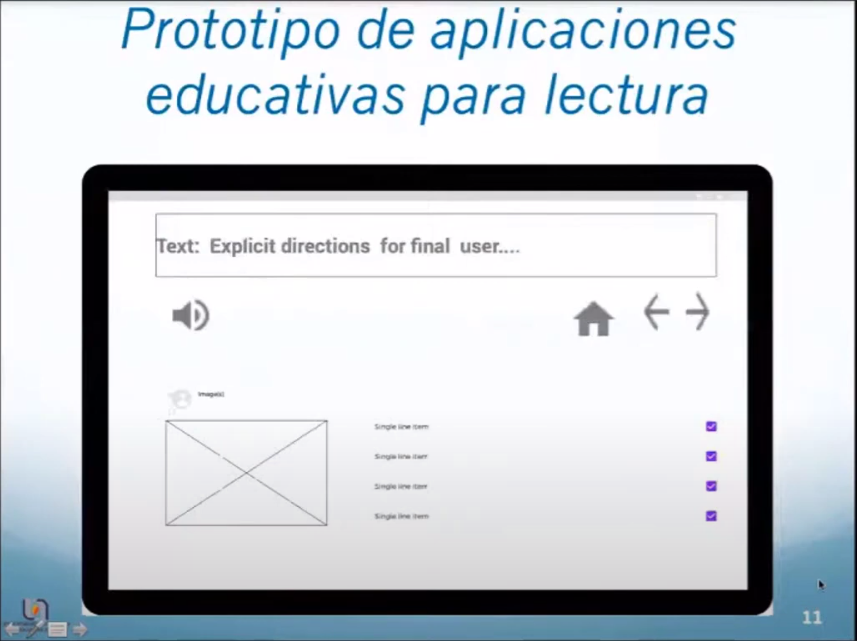
\includegraphics[width=0.8\textwidth]{ImagenLectura5.png}
    \end{figure}
\end{frame}

\begin{frame}
\frametitle{Capacitación Docente}
    \begin{figure}
    \centering
     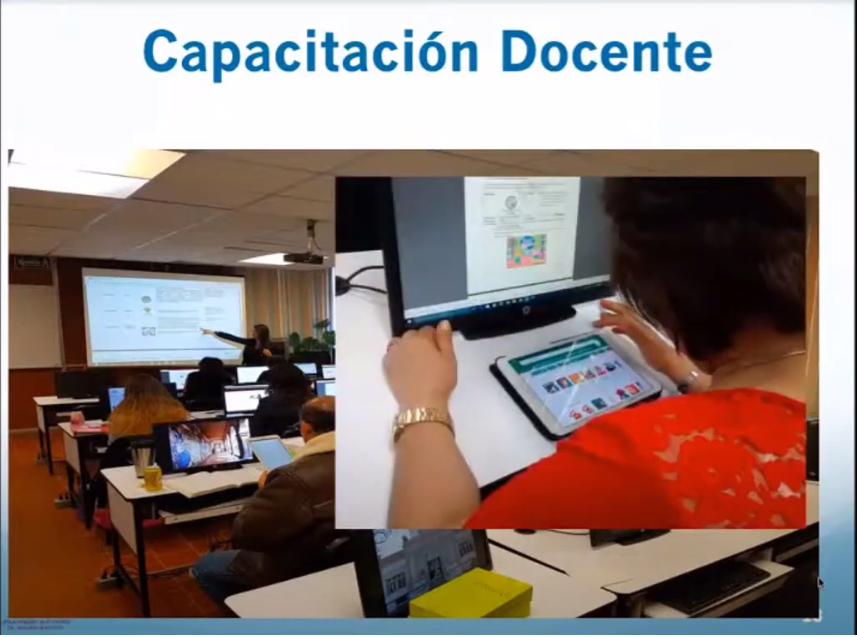
\includegraphics[width=0.8\textwidth]{ImagenLectura6.png}
    \end{figure}
\end{frame}

\begin{frame}
\frametitle{Requerimientos}
    \begin{figure}
    \centering
     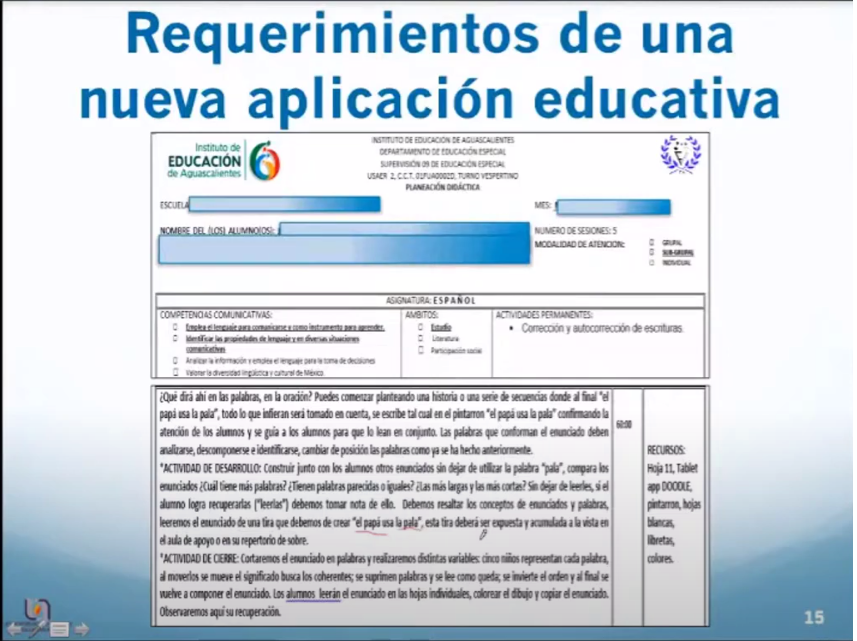
\includegraphics[width=0.8\textwidth]{ImagenLectura7.png}
    \end{figure}
\end{frame}

\begin{frame}
\frametitle{Grado de Lectura}
    \begin{figure}
    \centering
     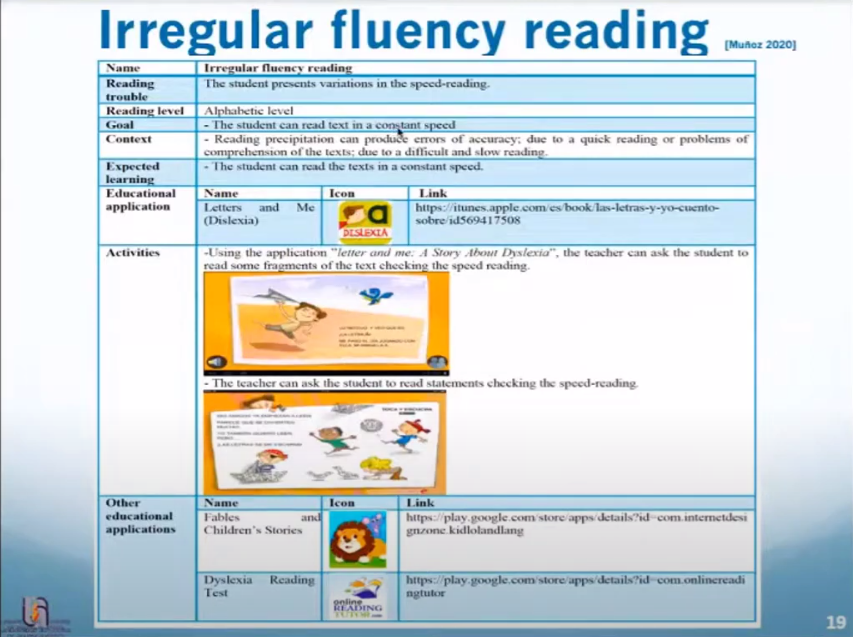
\includegraphics[width=0.8\textwidth]{ImagenLectura8.png}
    \end{figure}
\end{frame}

\begin{frame}
\frametitle{Pruebas de Uso}
    \begin{figure}
    \centering
     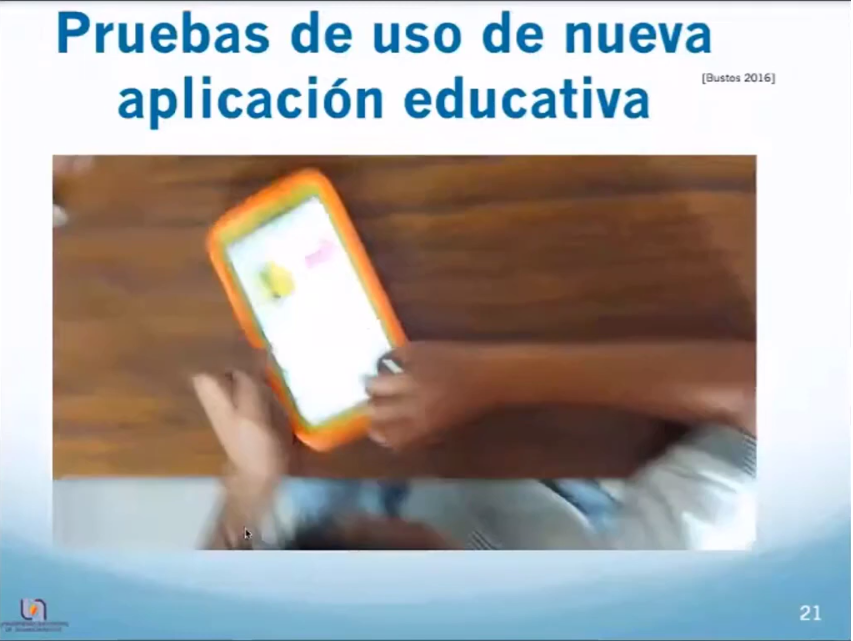
\includegraphics[width=0.8\textwidth]{ImagenLectura9.png}
    \end{figure}
\end{frame}

\begin{frame}
\frametitle{Resultados}
    \begin{figure}
    \centering
     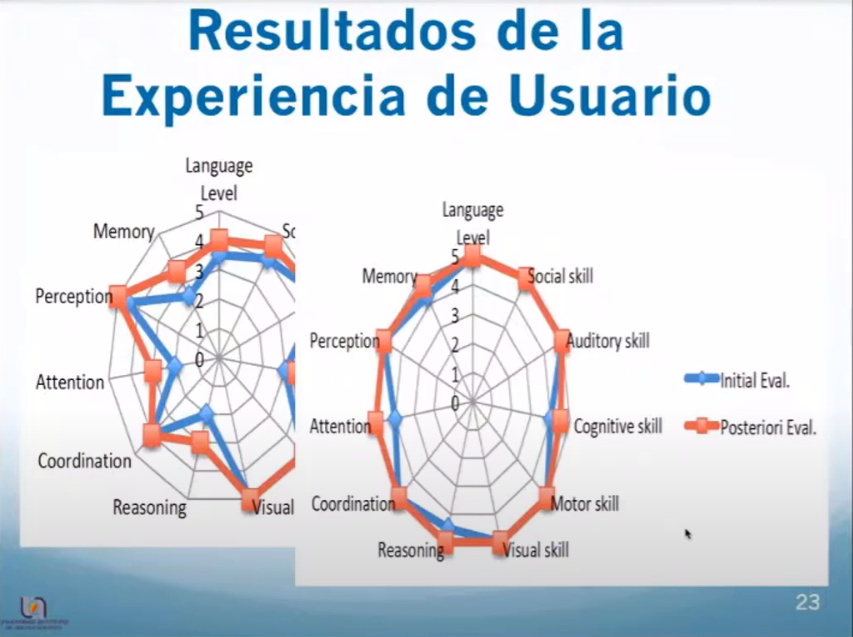
\includegraphics[width=0.8\textwidth]{ImagenLectura10.png}
    \end{figure}
\end{frame}

\begin{frame}
\frametitle{Aplicaciones con Kinect}
    \begin{figure}
    \centering
     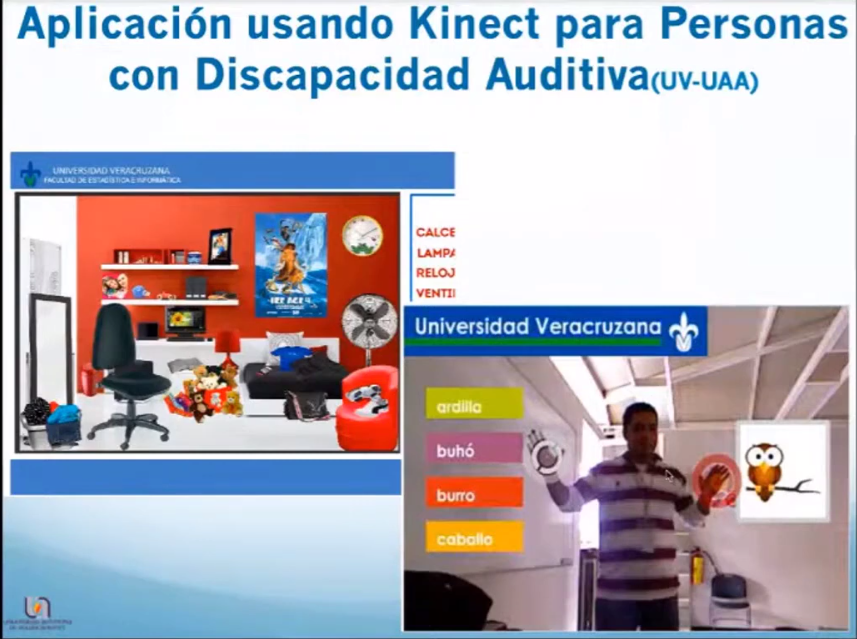
\includegraphics[width=0.8\textwidth]{ImagenLectura11.png}
    \end{figure}
\end{frame}

\begin{frame}
\frametitle{Audiolibros}
    \begin{figure}
    \centering
     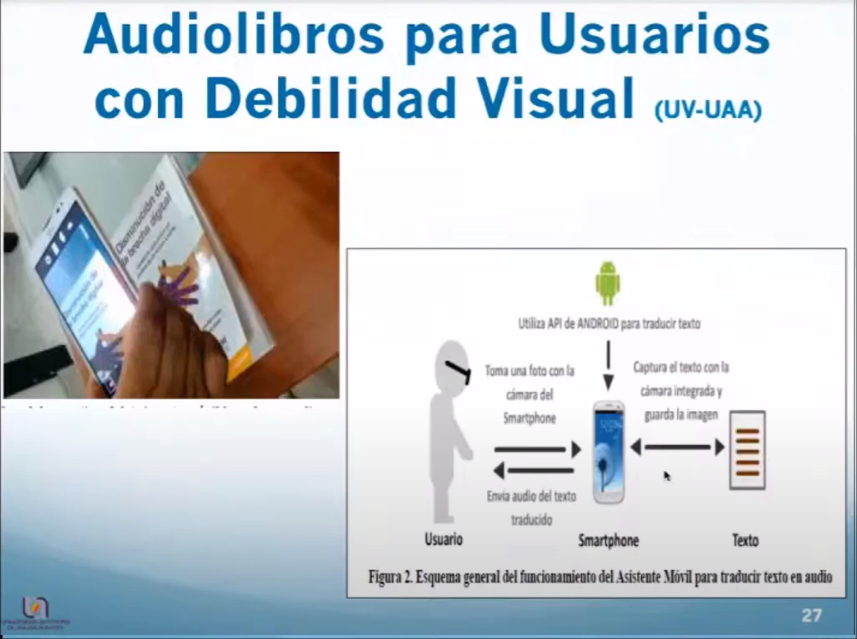
\includegraphics[width=0.8\textwidth]{ImagenLectura12.png}
    \end{figure}
\end{frame}

\section{Experiencia en apoyo a aprendizaje inclusivo de matematicas basicas}
\title{Experiencia en matemáticas básicas}
\begin{frame}
\frametitle{Experiencia en apoyo a aprendizaje inclusivo de matematicas basicas}
\end{frame}

\section{Conclusiones}
\begin{frame}
\frametitle{Conclusiones}
\end{frame}

\section{References}
%References frame
\begin{frame}
\frametitle{References}
\begin{itemize}
\item \href{https://www.youtube.com/watch?v=F0nOl4GRfC4&t=1577s}{J. Muñoz. Diseño de software interactivo educativo inclusivo - HCI 2020}
\end{itemize}
\end{frame}

\end{document}
